% ============================================================
%  Final Report — template
%  Modeled on the previous reports in assignments/publication_media
%  (ACM acmart / sigconf house style). Replace <PLACEHOLDER> text and
%  the example content; the structure, tables, figures, and equations
%  are illustrative and meant to be edited.
% ============================================================
\documentclass[sigconf,nonacm]{acmart}

% ── Packages (matching the previous reports) ──
\usepackage{graphicx}     % figures
\usepackage{booktabs}     % \toprule \midrule \bottomrule
\usepackage{float}        % [H] float placement
\usepackage{hyperref}     % \url, cross-refs
\usepackage{amsmath}      % equations
\usepackage{tikz}         % diagrams (delete if unused)
\usetikzlibrary{positioning, arrows.meta, fit, backgrounds, calc}

% ── ACM boilerplate: strip conference/copyright furniture ──
\settopmatter{printacmref=false, printfolios=true}
\setcopyright{none}
\renewcommand\footnotetextcopyrightpermission[1]{}
\pagestyle{plain}

% Avoid text protruding past the right margin (overfull hboxes) by allowing
% LaTeX a little extra inter-word stretch only when a line would overflow.
\setlength{\emergencystretch}{3em}

% Let large top floats share a page instead of deferring to the next.
\renewcommand{\topfraction}{0.9}
\renewcommand{\dbltopfraction}{0.9}
\renewcommand{\textfraction}{0.07}
\renewcommand{\floatpagefraction}{0.7}
\renewcommand{\dblfloatpagefraction}{0.7}

\begin{document}

% ────────────────────────────────────────────────────────────
%  Front matter
% ────────────────────────────────────────────────────────────
\title{Risk Estimation of Preeclampsia}

\author{Ahmed Khan}
\email{aekhan@ucdavis.edu}
\affiliation{%
  \institution{UC Davis}
  \city{Davis, CA}
  \country{USA}
}

\author{Lawrencedel Legaspi}
\email{lawlegaspi@ucdavis.edu}
\affiliation{%
  \institution{UC Davis}
  \city{Davis, CA}
  \country{USA}
}

\author{Selena Phu}
\email{slphu@ucdavis.edu}
\affiliation{%
  \institution{UC Davis}
  \city{Davis, CA}
  \country{USA}
}

\begin{abstract}
  % ── Code / data availability (optional — delete if not applicable) ──
  \noindent\textbf{Code Availability:} \url{https://github.com/AhmedKhan-GH/repnet}

  \medskip
  Reliably identifying preeclampsia, a leading cause of maternal and
  fetal morbidity, from routine clinical data remains challenging.
  Recent work has shown that preeclampsia leaves a detectable signature
  on the standard 12-lead electrocardiogram
  (ECG)~\cite{butler_ai-based_2024}, a cheap, non-invasive, and widely
  available test. We present \textit{RepNet}, a pair of
  machine-learning models that aim to identify preeclampsia directly from
  12-lead ECGs. RepNet-CNN is a compact,
  channel-independent convolutional neural network (29{,}490 parameters)
  in which all twelve leads pass through a shared-weight 1D backbone and
  are fused by a single linear layer; RepNet-RF is a decision-tree
  ensemble trained on interpretable ECG features extracted with NeuroKit2
  and GE MUSE-reported measurements. Both models were trained and evaluated on 2{,}178
  clinical 12-lead ECGs (335 preeclamptic, 15.4\% prevalence) from 1{,}383
  patients at UC Davis Health, using 30 patient-grouped 80/20 splits to
  prevent patient-level leakage. RepNet-CNN attains a mean AUROC of
  $0.709 \pm 0.049$ (best split 0.779), and RepNet-RF a mean AUROC of
  $0.757 \pm 0.039$. Gradient-based saliency and decision-tree feature
  importance independently converge on clinically established markers
  (QRS morphology, ST-segment changes, and the $T_{pe}$ interval), showing
  that both approaches recover known cardiac effects of preeclampsia and
  that 12-lead ECGs carry discriminative signal for low-cost screening.
\end{abstract}

\maketitle

% ════════════════════════════════════════════════════════════
\section{Introduction}
\label{sec:intro}

Preeclampsia is a hypertensive disorder of pregnancy and one of the leading
causes of maternal and fetal harm. It affects an estimated 2--8\% of
pregnancies worldwide~\cite{ozcan_preeclampsia_2025} and with related
hypertensive disorders claims more than 76,000 lives a
year~\cite{butler_ai-based_2024}. Left unmanaged it can progress rapidly to
eclampsia, organ failure, and death~\cite{mayo_clinic_preeclampsia_nodate}. Yet routine screening still relies on
blood pressure, urine protein, and blood panels that often catch the disorder
only once it is clinically apparent~\cite{noauthor_preeclampsia_2018}. The
burden falls hardest on low-resource settings where specialist obstetric care
is scarce and a cheap, widely available test would help most.

The standard 12-lead electrocardiogram (ECG) is a compelling candidate
for such a test. It is cheap, non-invasive, and already ubiquitous in
clinical practice. There is also a clear physiological reason to expect it
to carry information about preeclampsia: the disorder imposes measurable
cardiac stress that the ECG can capture. Raffaelli et al.\ found that
preeclamptic women exhibit altered ventricular repolarization and
increased QT dispersion on standard
ECG~\cite{raffaelli_pre-eclampsia_2014}. A 2025 systematic review and
meta-analysis of 57 studies quantified this effect, reporting that
third-trimester preeclampsia prolongs the heart-rate-corrected QT (QTc)
interval by 21.7~ms relative to normal
pregnancy~\cite{aboshady_qtc_2025}. Beyond repolarization, Angeli et al.\
report that left atrial abnormality on a standard ECG is associated with
a roughly fourfold increase in the risk of developing a hypertensive
disorder of pregnancy~\cite{angeli_novel_2015}.

To our knowledge, the only prior study to diagnose preeclampsia from ECG
waveforms is Butler et al., who trained a modified ResNet convolutional
neural network on raw 12-lead ECGs and identified preeclampsia with an
AUC of 0.85 on a holdout set and 0.81 on an external
cohort~\cite{butler_ai-based_2024}, building on an earlier demonstration
of the same approach~\cite{butler_electrocardiographic_2023}. Their
discussion points to two future improvements. One reduces the number of
leads; the other uses a single-lead (lead~I) model that smart wearables could
mimic. The first aligns with our own goal of cutting cost and complexity by
requiring fewer leads. Their follow-up work supports the second. There a
single-lead (lead~I) model predicts fatal coronary heart disease, and a
clinical ECG and an Apple Watch agree on its risk classification for 99\% of
participants~\cite{butler_feasibility_2024}. Whether a single-lead model could help our
task remains open, since several of our features cannot be computed from one
lead alone. More broadly, reviews of machine
learning for preeclampsia note that most models are built on
electronic-health-record features rather than ECG
waveforms~\cite{ozcan_preeclampsia_2025}.

Lead reduction is feasible in principle. Xue shows that a four-lead subset
(I, II, V2, and V4) fed into a deep neural network reproduces full 12-lead
morphology interpretations and detects abnormalities such as bundle branch
block, ischemia, and myocardial infarction about as
well~\cite{xue_does_2024}. Much of the diagnostic information thus survives
aggressive lead reduction. Whether this transfers to preeclampsia is unclear,
because the diagnosis is not tied to lead-specific morphology in the same way.
The result still bears on our setting, because the subset keeps the limb leads
I and II that several of our engineered features need, such as the mean
electrical axis~\cite{noauthor_visualising_nodate}.

Decision-tree models have likewise shown promise for preeclampsia, though
always from tabular clinical data rather than the ECG. Bülez et al.\
trained a LightGBM classifier on electronic health records and found
hemoglobin, age, and liver-enzyme levels (AST and ALT) to be the strongest
predictors, reaching an AUROC of 0.832~\cite{bulez_artificial_2024}. Zhang
et al.\ instead fit an XGBoost model to early-pregnancy urine metabolomics,
isolating seven biomarkers that detect preeclampsia with an AUROC of
0.856~\cite{zhang_development_2023}. No such model has yet been built on
features drawn from the ECG. Tree ensembles are also far cheaper to run
than convolutional networks. They may give up some accuracy, but that
efficiency makes them attractive for clinics with limited or aging hardware.

Against this backdrop we develop \textit{RepNet}, a pair of machine-learning
models that identify preeclampsia directly from 12-lead ECGs. We train and
evaluate both on an independent cohort of 2,178 clinical ECGs from 1,383
patients at UC Davis Health, of which 335 (15.4\%) are preeclamptic. The first
model, RepNet-CNN, is a compact channel-independent convolutional network of
29,490 parameters. Every lead passes through a single shared-weight 1D
backbone, and one linear layer fuses the resulting per-lead features. The
second, RepNet-RF, is a decision-tree ensemble trained on interpretable ECG
features extracted with NeuroKit2 and GE MUSE-reported measurements. We
evaluate both with patient-grouped cross-validation that guarantees no patient
appears in both training and test partitions.

% ════════════════════════════════════════════════════════════
\section{Dataset}
\label{sec:data}

RepNet was developed on a retrospective cohort of clinical 12-lead ECGs from
pregnant patients at UC Davis Health. Each recording is a standard 10-second,
12-lead ECG sampled at 500\,Hz and comes with the vendor (GE MUSE)
interpretation and a de-identified patient identifier. We label a recording
preeclamptic when its diagnosis is \emph{preeclampsia or other hypertensive
disorder of pregnancy} and normal otherwise. The raw export held 2,483
metadata entries, of which 2,191 had a matching waveform file. We then
discarded any recording with a non-finite sample, a flat lead (raw standard
deviation $\sigma_\ell < 10^{-4}$), or a missing patient identifier. This
removed 13 recordings and two patients and left a clean cohort of 2,178 ECGs
from 1,383 patients, of which 335 (15.4\%) are preeclamptic.
Table~\ref{tab:cohort} reports the cohort before and after this step. The data
is protected health information and is available only under IRB approval and a
data-use agreement.

\begin{table}[H]
\centering
\caption{UCDH cohort before and after removal of broken recordings.}
\label{tab:cohort}
\small
\begin{tabular}{@{}lrrr@{}}
\toprule
& \textbf{Before} & \textbf{Removed} & \textbf{After} \\
\midrule
Patients & 1{,}385 & 2 & 1{,}383 \\
ECG recordings & 2{,}191 & 13 & 2{,}178 \\
\midrule
Preeclamptic & 337 & 2 & 335 \\
Normal & 1{,}854 & 11 & 1{,}843 \\
Prevalence & 15.4\% & -- & 15.4\% \\
\bottomrule
\end{tabular}
\end{table}

Two properties of this cohort shape the rest of the paper. First, the classes
are heavily imbalanced. A trivial model that labels every recording normal is
already 84.6\% accurate while catching no cases, so we report threshold-free
measures (AUROC and AUPRC) rather than accuracy. Second, the 1,383 patients
contribute the 2,178 recordings unevenly (Table~\ref{tab:perpatient}). Most
appear once and 428 (31\%) appear more than once, with one patient
contributing as many as 16 and a mean of 1.6 overall. The label is assigned at
the patient level, so no patient carries conflicting labels, but a naive
recording-level split would still place the same patient in both training and
test data and inflate performance. We therefore group every split by patient
(Section~\ref{sec:methods}) so that no patient is seen during both training and
evaluation. We use scikit-learn's \texttt{StratifiedGroupKFold}~\cite{pedregosa_scikit-learn_2011}, which
partitions by patient while preserving the class ratio in each fold.

\begin{table}[H]
\centering
\caption{Distribution of ECG recordings per patient across the cohort.}
\label{tab:perpatient}
\small
\begin{tabular}{@{}lrr@{}}
\toprule
\textbf{Recordings/patient} & \textbf{Patients} & \textbf{Recordings} \\
\midrule
1 & 955 & 955 \\
2 & 257 & 514 \\
3 & 101 & 303 \\
4--5 & 47 & 202 \\
6--10 & 16 & 114 \\
11--16 & 7 & 90 \\
\midrule
\textbf{Total} & \textbf{1{,}383} & \textbf{2{,}178} \\
\bottomrule
\end{tabular}
\end{table}

\subsection{Preprocessing}
\label{sec:preproc}

Raw traces carry baseline wander (drift below $\sim$0.5\,Hz) on an arbitrary
amplitude scale. We remove it with a 4th-order zero-phase 0.5\,Hz high-pass~\cite{jia_preprocessing_2024, adam_comparative_2025}
and z-score each lead. Normalization is per lead because median amplitude
varies $\sim$2.2$\times$ across leads; a global scale would let the largest
leads dominate the shared backbone. We keep a plain mean/std z-score rather
than a robust one, since the within-lead distribution is heavy-tailed
(excess kurtosis $15.4$) by design: that tail is the QRS complex we must
preserve.

The spectrum, estimated with Welch's method~\cite{welch_use_1967}, fixes the
remaining choices. Power at 60\,Hz is only $0.62\times$ its neighbours, so
the notch is defensive rather than corrective, and $\sim$99\% of energy lies
below 40\,Hz, far under the 125\,Hz Nyquist of a 250\,Hz signal~\cite{shannon_communication_1949}.

The cohort arrives at two native sampling rates: 1{,}780 recordings at
500\,Hz (5{,}000 samples over the 10\,s strip) and 398 at 250\,Hz (2{,}500
samples). Because the high-pass and notch are specified in Hz, we first
resample the 2{,}500-sample records up to 5{,}000 so the filters act
identically on every recording, apply them, then decimate every record by
two to a uniform 250\,Hz (2{,}500 samples) for the model input. We
standardize \emph{down} to 250\,Hz rather than \emph{up} to 500\,Hz for three
reasons. The 125\,Hz Nyquist of 250\,Hz already sits far above the
$\sim$40\,Hz band where the energy concentrates, so no diagnostic content is
lost. The 398 lower-rate recordings are natively 250\,Hz, so upsampling the
whole cohort would fabricate high-frequency detail they never captured. And
halving the length to 2{,}500 samples halves the model's input, parameters,
and compute.

% ════════════════════════════════════════════════════════════
\section{Exploratory Data Analysis}
\label{sec:eda}

\subsection{Inter-Lead Structure}
\label{sec:eda-leads}

A \emph{channel-dependent} model mixes the twelve leads from its first layer
(a 2D convolution or attention block); a \emph{channel-independent} model
runs each lead through the same network separately and combines them only at
the end. Mixing earns its extra parameters only if the \emph{relationship
between leads} carries class information.

In plain terms, we ask whether preeclampsia changes how the leads relate to
one another. We measure each lead pair's tendency to move together (their
correlation). We then average those pairwise relationships separately over
preeclamptic and normal recordings and ask how much the two averages differ.
They barely differ: the inter-lead relationships are almost identical in the
two classes. This is a statement about the \emph{relationships}, not the
leads themselves: the leads are not all alike, but any given pair
co-varies in much the same way whether or not the patient is preeclamptic.
The rest of this subsection makes that measurement precise, building from a
single lead pair up to one number.

\emph{Two leads.} For leads $a$ and $b$ sampled at $t=1,\dots,T$, their
Pearson correlation measures whether they move alike:
\begin{equation}
r_{ab} = \frac{\sum_{t}(a_t-\bar a)(b_t-\bar b)}
              {\sqrt{\sum_{t}(a_t-\bar a)^2}\,\sqrt{\sum_{t}(b_t-\bar b)^2}}
       \in [-1,1],
\label{eq:pearson}
\end{equation}
with $r_{ab}=1$ in perfect lockstep, $-1$ mirrored, and $0$ unrelated. The
numerator is the covariance of the two leads, while the denominator divides
out each lead's own spread, so $r_{ab}$ captures agreement in \emph{shape}
regardless of amplitude: a lead and a scaled copy of it score $1$.

\emph{All pairs of one recording.} Stacking $r$ over every lead pair gives
that recording's $12\times12$ correlation matrix, with unit diagonal:
\begin{equation}
C^{(n)}_{ij} = r_{ij}, \qquad i,j \in \{1,\dots,12\}, \quad C^{(n)}_{ii}=1.
\label{eq:cmat}
\end{equation}
The matrix is symmetric ($C^{(n)}_{ij}=C^{(n)}_{ji}$), so its content is the
$66$ distinct off-diagonal correlations.
Figure~\ref{fig:synth} shows these two steps on four synthetic leads.

\begin{figure}[t]
\centering
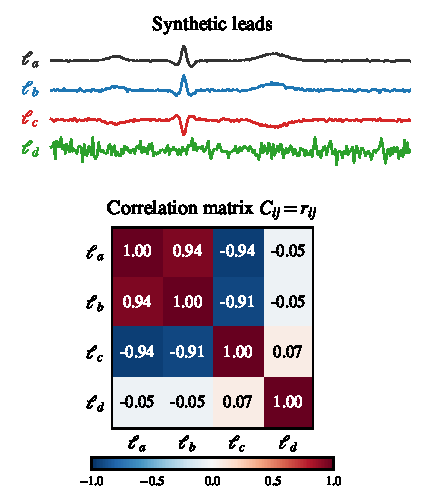
\includegraphics[width=\columnwidth]{figures/synthetic_corr.pdf}
\caption{The pairwise operation on four synthetic leads. $\ell_b$ tracks
$\ell_a$ ($r=0.94$), $\ell_c$ is its inverse ($r=-0.94$), and $\ell_d$ is
unrelated ($r=-0.05$); these values populate the correlation matrix $C$
(Eqs.~\eqref{eq:pearson}--\eqref{eq:cmat}), which has a unit diagonal.}
\label{fig:synth}
\end{figure}

\emph{Each class.} Averaging over recordings within a class gives its
typical coupling:
\begin{equation}
\bar{C}_{\mathrm{PE}} = \frac{1}{N_{\mathrm{PE}}}\!\sum_{n\in\mathrm{PE}}\! C^{(n)},
\qquad
\bar{C}_{\mathrm{N}}  = \frac{1}{N_{\mathrm{N}}}\!\sum_{n\in\mathrm{N}}\! C^{(n)}.
\label{eq:cbar}
\end{equation}
Here $N_{\mathrm{PE}}$ and $N_{\mathrm{N}}$ count the recordings in each
class; averaging cancels recording-specific noise and leaves the coupling
pattern typical of that class.

\emph{Disease effect, per pair.} Their entry-wise difference isolates how
each lead pair's coupling shifts with disease:
\begin{equation}
D = \bar{C}_{\mathrm{PE}} - \bar{C}_{\mathrm{N}}, \qquad
D_{ij} = \text{change in lead } i\text{--}j \text{ coupling}.
\label{eq:diff}
\end{equation}
Since both class matrices have a unit diagonal, $D$ has a zero diagonal: a
positive off-diagonal entry marks a lead pair that grows \emph{more}
correlated under preeclampsia, a negative one a pair that decouples.

\emph{One number.} The Frobenius norm (the Euclidean length of the matrix
read as a flat list of entries) collapses all of $D$ into a single
nonnegative magnitude~\cite{horn_matrix_2012}:
\begin{equation}
\lVert D \rVert_F = \sqrt{\sum_{i=1}^{12}\sum_{j=1}^{12} D_{ij}^{2}}
                  = 0.979 .
\label{eq:frob}
\end{equation}

Equations~\eqref{eq:diff}--\eqref{eq:frob} make the conclusion concrete:
each $D_{ij}$ is a verdict on whether one lead pair couples the same way in
both classes, and the norm sums those per-pair verdicts into one score. It is $0$ only if
\emph{every} pair is identical. Here it is $0.979$: the off-diagonal
entries average just $0.073$ and never exceed $0.174$ on the $[-1,1]$ scale,
and the two class matrices are indistinguishable by eye
(Fig.~\ref{fig:corr}). The leads co-vary almost identically with or without
preeclampsia.

A channel-dependent model would therefore spend parameters on cross-lead
structure that barely differs between classes; the discriminative signal
must instead live \emph{within} each lead. We process every lead
independently through one shared-weight 1D backbone and fuse only at the
final linear layer (Section~\ref{sec:methods}). A per-lead RMS test confirms
no lead carries the signal alone (only $1/12$ clears $p<0.05$), so
shared weights, not lead-specific pathways, are the right choice.

\begin{figure}[H]
\centering
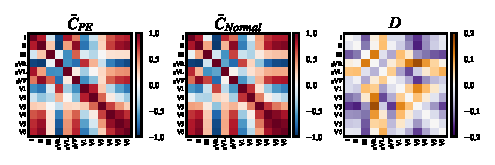
\includegraphics[width=\columnwidth]{figures/lead_corr_diff.pdf}
\caption{Class-average inter-lead correlation matrices for preeclamptic
($\bar{C}_{\mathrm{PE}}$) and normal ($\bar{C}_{\mathrm{N}}$) recordings and
their difference $D$ on the real cohort. The two class matrices are nearly
identical and $D$ is near zero everywhere (note the $\pm0.2$ scale), giving
$\lVert D\rVert_F = 0.979$.}
\label{fig:corr}
\end{figure}

\subsection{Temporal Scale and Alignment}
\label{sec:eda-scale}

The shape of the per-lead backbone (where in time to look, and how
widely) follows from two questions about the time axis.

\emph{Is the signal tied to a fixed position?} A classifier that flattens
the time axis treats absolute position as meaningful; one that pools over
time does not. We test which is appropriate by comparing the classes
sample-by-sample on a common clock. The recordings are not R-peak aligned,
so averaging washes out beat morphology: the class-mean waveform of lead~II
hovers near zero for both classes, while the within-class standard deviation
is an order of magnitude larger and the two $\pm$std bands overlap almost
completely (Fig.~\ref{fig:temporal}, top). The between-class mean difference
is correspondingly small (at most $0.21$ against a within-class std of
$\approx 1.0$) and \emph{smeared across the entire ten-second strip}
rather than concentrated at any latency (Fig.~\ref{fig:temporal}, bottom).
The discriminative cue is therefore \emph{local waveform morphology wherever
it occurs}, not its absolute position. This calls for convolutions, which
detect a pattern regardless of where it sits, followed by \emph{global
average pooling}, which collapses the time axis and makes the model
invariant to where in the strip a beat falls.

\begin{figure}[t]
\centering
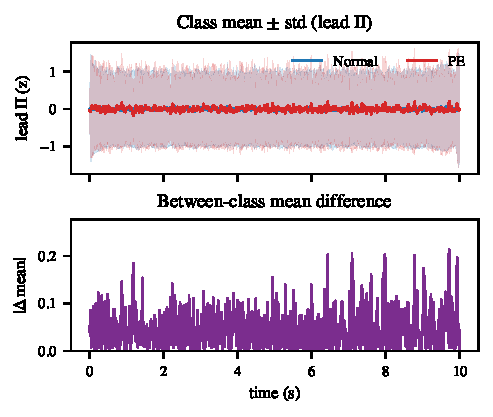
\includegraphics[width=\columnwidth]{figures/temporal_alignment.pdf}
\caption{Lead~II on a common clock. Top: the class-mean waveforms
(PE red, Normal blue) are washed out and their $\pm$std bands overlap
almost entirely, so within-class variation dominates. Bottom: the
between-class mean difference stays small and is spread across the whole
strip, with no localized peak: the signal is not tied to a fixed
position.}
\label{fig:temporal}
\end{figure}

\emph{At what temporal scale?} The morphology that carries the signal is the
PQRST complex of a single beat. At $60$--$100$ beats per minute a cardiac
cycle lasts $600$--$1000$\,ms, and the diagnostic waveform (the P wave,
QRS complex, ST segment, and T wave) occupies roughly its first
$400$\,ms~\cite{surawicz_chous_2008}. This fixes a requirement on the backbone: each per-lead feature
should integrate about one complete PQRST complex, so that a repolarization
change can be read relative to the QRS that precedes it. The markers
implicated in preeclampsia (QT, $T_{pe}$, and ST shifts)~\cite{raffaelli_pre-eclampsia_2014, aboshady_qtc_2025} are all defined
this way. Section~\ref{sec:cnn-arch} shows that the chosen kernels meet this
$\sim$one-cycle target with a $444$\,ms receptive field, after which global
average pooling aggregates the per-beat summaries across the whole strip.

\subsection{Spectral Separability}
\label{sec:eda-psd}

A natural alternative to learning from morphology is to classify from the
signal's frequency content. We checked whether the classes separate in the
power spectrum by estimating each recording's Welch periodogram (averaged
over leads) and asking, at each frequency, how well a single bin's power
distinguishes the two classes. They do not (Fig.~\ref{fig:psd}). Shown
before the $60$\,Hz notch, the class-average spectra are nearly identical and
carry no prominent mains peak, and per-bin separability hovers at chance
across the spectrum; the best-performing range ($1$--$5$\,Hz) reaches only
an AUROC of $0.54$. This is expected: preeclampsia alters waveform
\emph{morphology and relative timing} (T-wave shape, intervals defined
against the QRS)~\cite{raffaelli_pre-eclampsia_2014}, which a power spectrum discards along with phase. The
result confirms that the discriminative signal is morphological, supporting a
model that convolves over the waveform rather than one built on spectral
features.

\begin{figure}[t]
\centering
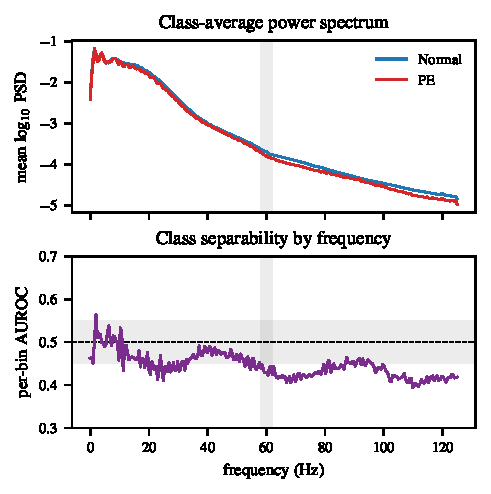
\includegraphics[width=\columnwidth]{figures/psd_class.pdf}
\caption{The classes do not separate in the frequency domain; spectra are
shown \emph{before} the $60$\,Hz notch. Top: the class-average power spectra
(PE red, Normal blue) are nearly identical, with no prominent mains peak at
$60$\,Hz (shaded). Bottom: the AUROC of each frequency bin's power for
separating the classes stays within the chance band ($0.45$--$0.55$) across
the spectrum.}
\label{fig:psd}
\end{figure}

% ════════════════════════════════════════════════════════════
\section{Methods}
\label{sec:methods}

RepNet comprises two models that approach preeclampsia identification from
opposite ends of the feature-engineering spectrum. They share only the cohort
(Section~\ref{sec:data}) and the patient-grouped cross-validation used to
evaluate them. A recording is $x \in \mathbb{R}^{12\times2500}$ (twelve leads,
$2{,}500$ samples at $250$\,Hz) with a binary label, and both estimate
$\mathbb{P}(\text{preeclampsia}\mid x)$; they differ in what they look at.

RepNet-CNN consumes the raw waveform and learns its own features through the
shared per-lead backbone motivated in Section~\ref{sec:eda}. RepNet-RF is an entirely separate model that does not
use the raw waveform at all; it classifies a vector of \emph{manually
derived} ECG features. Using NeuroKit2~\cite{makowski_neurokit2_2021}, it computes a fixed set of clinically defined measurements
(QT dispersion, the $T_{pe}$ interval and its rate-corrected ratios,
ST-segment elevation and depression, P-wave dispersion, and the frontal
QRS--T axis) chosen with our clinical advisors to capture repolarization
markers the vendor pipeline omits. It then combines these with the $656$
measurements the GE MUSE system already reports for each recording. A
decision-tree ensemble classifies the resulting vector: a random forest~\cite{breiman_random_2001} voted
with logistic-regression and support-vector-machine~\cite{cortes_support-vector_1995} classifiers. Built from different representations of
the same signal, the two models also serve as a cross-check: where a learned
model and a feature-based one agree, the underlying signal is more credible
than either alone would establish.

\subsection{RepNet-CNN}

\subsubsection{Architecture}
\label{sec:cnn-arch}

RepNet-CNN realizes the two findings of Section~\ref{sec:eda}: it processes
each lead independently through one shared-weight backbone
(Section~\ref{sec:eda-leads}), sized to see a single heartbeat
(Section~\ref{sec:eda-scale}). The input is reshaped from $(12,2500)$ to
$(12,1,2500)$ so the same backbone is applied to every lead. That backbone is
three stages of $\text{Conv1d}\to\text{BatchNorm}\to\text{Mish}$
(Fig.~\ref{fig:convblock}) with channel widths $16\to32\to48$, kernels $31$,
$21$, $11$, and stride $2$ throughout. An adaptive average pool collapses
each lead to a $48$-dimensional vector; the twelve vectors are concatenated
into a $576$-dimensional representation and mapped to logits by a single
$\mathrm{Dropout}(0.15)$, $\mathrm{Linear}(576,2)$ head. Because the backbone
weights are shared across all twelve leads, the model totals only
$29{,}490$ parameters; the full network is diagrammed in
Appendix~\ref{appendix:cnn} (Fig.~\ref{fig:arch}).

\paragraph{Receptive field.}
The backbone must \emph{see} a full PQRST complex to meet the $\sim$one-cycle
requirement of Section~\ref{sec:eda-scale}. For a stack of 1D convolutions
the receptive field follows the recurrence
\begin{equation}
\mathrm{RF}_\ell = \mathrm{RF}_{\ell-1} + (k_\ell - 1)\,J_{\ell-1},
\qquad
J_\ell = \prod_{j=1}^{\ell} s_j ,
\label{eq:rf}
\end{equation}
where $k_\ell$ and $s_\ell$ are the kernel size and stride of layer $\ell$,
$J_\ell$ is the cumulative stride (the \emph{jump} between adjacent outputs),
and $\mathrm{RF}_0 = J_0 = 1$. Each stride-$2$ layer doubles the jump, so the
$(k_\ell-1)\,J_{\ell-1}$ term grows geometrically and a few layers span a
wide field cheaply: the same $111$-sample reach would need a single
$111$-tap kernel versus the $31{+}21{+}11=63$ taps used here. The field
builds up as in Table~\ref{tab:rf}, reaching $111$ samples ($444$\,ms at
$250$\,Hz) by the third stage, about one cardiac cycle. This bounds only
the convolutional view; the adaptive average pool then spans the full
$2{,}500$-sample ($10$\,s) input, aggregating per-beat summaries over all
ten-to-sixteen beats before the leads are fused.

\begin{table}[H]
\centering
\caption{Receptive-field buildup of the per-lead backbone, applying
Eq.~\eqref{eq:rf} layer by layer.}
\label{tab:rf}
\small
\begin{tabular}{@{}lccccc@{}}
\toprule
\textbf{Layer} & $k_\ell$ & $s_\ell$ & $J_{\ell-1}$ & $\mathrm{RF}_\ell$ (samp.) & (ms) \\
\midrule
Input  & --& --& 1 & 1   & 4   \\
Conv 1 & 31 & 2  & 1 & 31  & 124 \\
Conv 2 & 21 & 2  & 2 & 71  & 284 \\
Conv 3 & 11 & 2  & 4 & 111 & 444 \\
\bottomrule
\end{tabular}
\end{table}

\subsubsection{Training}
\label{sec:cnn-train}

A fresh model is trained for each split. The objective is a focal
cross-entropy~\cite{lin_focal_2017} with focusing parameter $\gamma=1$ and label smoothing $0.05$,
\begin{equation}
\mathcal{L} = (1 - p_t)^{\gamma}\,\mathrm{CE}(y,\hat{y}),
\label{eq:focal}
\end{equation}
where $p_t$ is the model's probability for the true class; the
$(1-p_t)^{\gamma}$ factor down-weights already-confident examples. We apply
no explicit class weighting: the $15.4\%$ positive rate is handled instead by
this down-weighting together with mixup~\cite{zhang_mixup_2018} and heavy augmentation, which enlarge
the effective positive set rather than re-balance the loss. With probability
$0.5$ each batch is mixed up: two examples and their labels blended
linearly with $\lambda \sim \mathrm{Beta}(0.2, 0.2)$.

We optimize with AdamW~\cite{loshchilov_decoupled_2019} (learning rate $1.2\times10^{-3}$, weight decay
$5\times10^{-3}$) under a cosine schedule annealing to $10^{-6}$ over the
$80$-epoch budget, with batch size $64$ and two-step gradient accumulation
(effective batch $128$). Training stops early once the validation AUROC has
not improved for $20$ epochs, and the best-AUROC weights are restored.
Validation uses the inner fold of the patient-grouped split
(Section~\ref{sec:data}); no test data is seen during training, and a single
model is trained per split (no bagging).

\paragraph{Learning-rate schedule.}
The learning rate is not held fixed but annealed with a cosine
schedule~\cite{loshchilov_sgdr_2017}. Indexing epochs by $t=0,1,\dots,T_{\max}$,
the rate at epoch $t$ is
\begin{equation}
\eta_t = \eta_{\min} + \tfrac{1}{2}\,(\eta_{\max} - \eta_{\min})
         \left(1 + \cos\!\frac{\pi t}{T_{\max}}\right),
\label{eq:cosine}
\end{equation}
which traces one half-period of a cosine from the initial rate
$\eta_{\max}=1.2\times10^{-3}$ at $t=0$ down to the floor
$\eta_{\min}=10^{-6}$ at $t=T_{\max}$. We set $T_{\max}=80$ epochs (matching
the epoch budget) and step the schedule once per epoch
(\texttt{CosineAnnealingLR} in the released code). The cosine shape gives a
deliberately uneven decay: the rate is nearly flat early on, so the model
takes large, exploratory steps while the loss surface is far from any
minimum; it falls fastest through the middle epochs; then it flattens again
near the floor, so late updates are small and the weights settle into a
minimum rather than bouncing around it. Compared with a fixed rate this
trades early speed for late stability without manual step-decay tuning, and
compared with a linear decay the flat tails spend more budget at the two
rates that matter most: high for exploration, low for convergence. In
practice early stopping (patience $20$) usually halts a split before epoch
$80$, so the rate typically reaches the lower-middle of the curve rather than
the $10^{-6}$ floor; $T_{\max}$ therefore sets the \emph{shape} of the decay,
not a guaranteed endpoint. We use a single cosine run with no warm restarts.

\paragraph{Activation.}
Each backbone stage uses the Mish activation~\cite{misra_mish_2020} in place
of the usual ReLU,
\begin{equation}
\mathrm{Mish}(x) = x\,\tanh\!\big(\operatorname{softplus}(x)\big)
                 = x\,\tanh\!\big(\ln(1+e^{x})\big),
\label{eq:mish}
\end{equation}
the self-gated form already shown per block in Fig.~\ref{fig:convblock}.
Two properties motivate the choice over ReLU, both bearing on how gradients
flow during training. First, Mish is smooth and continuously differentiable
everywhere, whereas ReLU has a non-differentiable kink at the origin and a
flat zero branch; the smoother response gives a better-conditioned loss
surface and non-vanishing gradients through the negative regime. Second, Mish
is non-monotonic and bounded below (it dips to $\approx-0.31$ before rising),
so a unit driven slightly negative still passes a small signal and a non-zero
gradient. ReLU instead zeros every negative pre-activation and its gradient
there, so units that drift negative can stop updating entirely, the
``dying ReLU'' failure mode. This matters most for a model this small: with
only $29{,}490$ parameters there is little spare capacity to lose to dead
units. Mish was introduced as a self-regularizing, non-monotonic activation
and reported to improve accuracy over ReLU and Swish across a range of vision
benchmarks~\cite{misra_mish_2020}; we adopt it for these properties rather
than from an in-house activation ablation.

Every training waveform is augmented on the fly with seven stochastic,
label-preserving transforms (Table~\ref{tab:aug}), each mimicking a plausible
source of recording variation. Together they expand the effective training
set, valuable given only $\sim$$230$ positive recordings per training
fold.

\begin{table}[H]
\centering
\caption{The seven on-the-fly training augmentations, applied to each
$250$\,Hz waveform with probability $p$.}
\label{tab:aug}
\small
\begin{tabular}{@{}llp{3.4cm}@{}}
\toprule
\textbf{Augmentation} & \textbf{$p$} & \textbf{Parameters} \\
\midrule
Gaussian noise          & 0.50 & $\sigma \in [0.01, 0.05]$ \\
Amplitude scale (per lead) & 0.50 & $\pm15\%$ \\
Time shift (circular)   & 0.30 & $\pm150$ samples \\
Lead dropout            & 0.10 & each lead zeroed w.p.\ $0.12$ \\
Cutout                  & 0.25 & zero a $50$--$200$-sample window \\
Baseline wander         & 0.20 & sine, $0.05$--$0.5$\,Hz, amplitude $\le 0.2$ \\
Resample / time-warp    & 0.10 & rate $1 \pm 0.05$ \\
\bottomrule
\end{tabular}
\end{table}

\subsection{RepNet-RF}
\label{sec:rf}

\subsubsection{Feature Engineering}

RepNet-RF classifies hand-engineered ECG features rather than the raw
waveform. Each of the $2{,}191$ recordings that has a waveform arrives with
$656$ measurements already computed by the GE MUSE system, which we call the
\emph{metadata}; with guidance from our clinical advisor Dr.~Lihong Mo, we
additionally extract features linked to preeclampsia that MUSE does not
report. NeuroKit2 feature extraction fails on a small number of recordings
(for example when delineation returns missing landmarks), and those are
dropped; to keep the comparison fair, the MUSE-derived features drop the same
recordings. Table~\ref{tab:rf-cohort} gives the resulting counts for the full
(unbalanced) cohort and for a class-balanced subset used in some experiments.

\begin{table}[H]
\centering
\caption{Recordings used by RepNet-RF, before and after dropping cases where
NeuroKit2 extraction failed (preeclamptic\,/\,normal).}
\label{tab:rf-cohort}
\small
\begin{tabular}{@{}lccc@{}}
\toprule
\textbf{Dataset} & \textbf{Original} & \textbf{Dropped} & \textbf{Final} \\
\midrule
Unbalanced & 337 / 1854 & 8 / 24 & 329 / 1830 \\
Balanced   & 187 / 182  & 6 / 1  & 181 / 181  \\
\bottomrule
\end{tabular}
\end{table}

NeuroKit2 provides routines for cleaning ECG signals and locating fiducial
landmarks. Because raw traces drift from a common baseline, a baseline-wander
filter is applied before delineation, after which we compute the features in
Table~\ref{tab:rf-neuro}. Our graduate mentor Hana Shaik had previously
implemented the ST--T abnormality features for detecting regional wall motion
abnormalities~\cite{joshi_linking_2025}; we validated our implementation
against hers and on the Nightingale ECG dataset, confirming the clinical
interpretation of each formula.

The frontal QRS and T axes were the hardest to compute. We implement the QRS
axis two ways: an isoelectric method that locates the isoelectric lead and
reads $\pm90^\circ$ from the sign of the perpendicular lead, and a direct
$\arctan$ formula that returns a specific
angle~\cite{noauthor_calculating_2022, noauthor_visualising_nodate},
though in clinical practice small angular differences are
insignificant~\cite{noauthor_calculating_2022}. The T axis uses the
analogous $\arctan$ form~\cite{scherer_abnormal_2009}, and the frontal
QRS--T angle is their absolute difference. Dr.~Ebong, a UC Davis Health
cardiologist, is evaluating the accuracy of these implementations.

\subsubsection{Comparison with MUSE Features}

To check the NeuroKit features, we recomputed the same quantities from the
MUSE metadata (Table~\ref{tab:rf-muse}) on the identical set of recordings.
Averaged across recordings, the NeuroKit values are consistently lower than
the MUSE values. We briefly trialed an alternative library, ECGDataKit, whose
functions more closely mirror MUSE: it gave a closer median R-peak amplitude
but failed on the $250$\,Hz recordings and offered fewer feature routines, so
we retained NeuroKit2.

The NeuroKit2 and MUSE feature definitions are listed in
Appendix~\ref{appendix:features}.

\subsubsection{Classifier}

Each feature set is classified by a random forest inside a stratified group
$k$-fold split keyed on the obfuscated patient MRN, which prevents leakage,
with a random undersampler applied within the training folds~\cite{batista_study_2004, lemaitre_imbalanced-learn_2017}. We evaluate
three feature sources (the NeuroKit2 features, their MUSE-reported
counterparts, and either combined with the full MUSE metadata) and report
their performance in Section~\ref{sec:results-rf}.

\subsection{Evaluation Protocol}
\label{sec:eval}

Both models are evaluated with \emph{patient-grouped, stratified}
cross-validation built on scikit-learn's \texttt{StratifiedGroupKFold}.
Grouping on the obfuscated patient MRN guarantees that no patient appears in
both a training and a test partition: without it, the $428$ patients with
multiple recordings (Section~\ref{sec:data}) would leak identity across the
split and inflate every metric. Stratification holds the $15.4\%$
preeclampsia prevalence fixed in every fold, so each test set reflects the
clinical base rate. The two models differ only in how the folds are used.

\paragraph{RepNet-RF} A single five-fold \texttt{StratifiedGroupKFold}
(\texttt{shuffle=True}, fixed random seed): each of the five folds serves
once as the $20\%$ held-out test set while the model trains on the other
four, with a \texttt{RandomUnderSampler} balancing the training folds. The
reported metrics are the mean over the five test folds.

\paragraph{RepNet-CNN} Rather than a single five-fold pass, the CNN is
evaluated over \emph{thirty independent} patient-grouped $80/20$ splits, each
seeded by $s_i = 7i + 1000$ for split $i = 0,\dots,29$. Within a split, an
outer \texttt{StratifiedGroupKFold} (five folds, \texttt{random\_state}~$=s_i$)
supplies one fold as the $20\%$ held-out test set and the remaining $80\%$ as
a development set; an inner \texttt{StratifiedGroupKFold} (eight folds,
\texttt{random\_state}~$=s_i+1$) on the development set carves off a
validation fold for early stopping (Section~\ref{sec:cnn-train}). Each split
trains a fresh model, and we report the mean $\pm$ standard deviation of every
metric across the thirty splits. The randomized seeding turns evaluation into
a distribution rather than a single fold: the spread directly estimates
run-to-run stability on this small, imbalanced cohort, and the best and
median splits supply the released checkpoints.

For both models we report threshold-free discrimination (AUROC and AUPRC,
the latter against the $0.154$ prevalence baseline) together with two
operating points: Youden's $J$~\cite{youden_index_1950}, which maximizes
sensitivity~$+$~specificity~$-1$, and a screening point that fixes
sensitivity at $\geq 80\%$ and reports the resulting specificity and negative
predictive value.

% ════════════════════════════════════════════════════════════
\section{Results}
\label{sec:results}

\subsection{RepNet-CNN}
\label{sec:results-cnn}

RepNet-CNN attains a mean AUROC of $0.709 \pm 0.049$ over the $30$
patient-grouped splits (Table~\ref{tab:cnn-results}). Scores range from
$0.594$ on the hardest split to $0.779$ on the easiest, a spread that
justifies reporting the distribution rather than a single fold. Its AUPRC of
$0.342 \pm 0.075$ sits well above the $0.154$ no-skill baseline set by the
prevalence. The model works best as a rule-out screen. At a threshold fixed to
$80\%$ sensitivity it holds a negative predictive value of $0.928 \pm 0.019$,
its most stable metric across splits, so a negative prediction meaningfully
lowers the probability of preeclampsia. Its specificity ($0.50$) and precision
are more modest, so a positive prediction warrants confirmatory assessment
rather than standing alone.

\begin{table}[H]
\centering
\caption{RepNet-CNN performance by operating point over $30$ patient-grouped
splits (percent, mean $\pm$ std). AUROC and AUPRC are threshold-free.}
\label{tab:cnn-results}
\footnotesize
\setlength{\tabcolsep}{2.7pt}
\resizebox{\columnwidth}{!}{%
\begin{tabular}{@{}lcccccc@{}}
\toprule
\textbf{Operating point} & \textbf{AUROC} & \textbf{AUPRC} & \textbf{Spec.} & \textbf{Sens.} & \textbf{Bal.\ Acc.} & \textbf{F1} \\
\midrule
Youden's $J$ ($\tau{=}0.61$)       & 70.9$\pm$4.9 & 34.2$\pm$7.5 & 62.7$\pm$12.6 & 73.0$\pm$9.2 & 67.9$\pm$3.8 & 40.4$\pm$6.9 \\
Sens.\ $\geq 80\%$ ($\tau{=}0.55$) & 70.9$\pm$4.9 & 34.2$\pm$7.5 & 49.6$\pm$8.9 & \textbf{80.7$\pm$0.5} & 65.1$\pm$4.4 & 36.7$\pm$6.1 \\
\bottomrule
\end{tabular}}
\end{table}

The ROC and precision--recall curves on the best split (AUROC $0.779$,
average precision $0.485$ against the $0.16$ prevalence baseline) are shown in
Appendix~\ref{appendix:cnn} (Fig.~\ref{fig:cnn-roc}). To see \emph{where}
the network looks, we attribute the preeclampsia logit back to the Lead~II
waveform with Integrated Gradients~\cite{sundararajan_axiomatic_2017} and Grad-CAM~\cite{selvaraju_grad-cam_2020} (Fig.~\ref{fig:cnn-saliency}).
On a confident true positive the attribution toward preeclampsia concentrates
on the QRS complexes and ST segments, and it reverses sign on a true negative;
the network keys on clinically meaningful morphology rather than spurious
artefacts.

\subsection{RepNet-RF}
\label{sec:results-rf}

Despite the systematic offset between the libraries, the NeuroKit- and
MUSE-derived features perform comparably (Table~\ref{tab:rf-perf1}): NeuroKit
under-reports values but does so consistently, so the classifier is largely
unaffected. Adding the extracted features to the full MUSE metadata expands
the set to $721$ features ($723$ with NeuroKit) and improves performance
(Table~\ref{tab:rf-perf2}), although a model trained on the metadata alone
scored slightly higher, a hint that the enlarged feature set begins to
overfit.

\begin{table}[H]
\centering
\caption{Random-forest performance with NeuroKit2- vs MUSE-derived features
(percent).}
\label{tab:rf-perf1}
\footnotesize
\setlength{\tabcolsep}{2.7pt}
\begin{tabular}{@{}lccccccc@{}}
\toprule
\textbf{Features} & AUROC & AUPRC & Spec. & Sens. & Acc. & Prec. & F1 \\
\midrule
Balanced, NeuroKit   & 66.22 & 67.53 & 66.26 & 57.49 & 61.87 & 62.99 & 59.98 \\
Balanced, MUSE       & 62.47 & 65.66 & 60.27 & 59.73 & 59.95 & 60.22 & 59.75 \\
Unbalanced, NeuroKit & 63.19 & 22.62 & 63.83 & 54.73 & 62.44 & 21.33 & 30.67 \\
Unbalanced, MUSE     & 64.25 & 24.68 & 64.75 & 55.33 & 63.32 & 22.03 & 31.44 \\
\bottomrule
\end{tabular}
\end{table}

\begin{table}[H]
\centering
\caption{Performance when the extracted features are added to the full MUSE
metadata (percent).}
\label{tab:rf-perf2}
\footnotesize
\setlength{\tabcolsep}{2.7pt}
\begin{tabular}{@{}lccccccc@{}}
\toprule
\textbf{Features} & AUROC & AUPRC & Spec. & Sens. & Acc. & Prec. & F1 \\
\midrule
MUSE\,+\,NeuroKit, bal.\    & 70.37 & 72.94 & 67.92 & 63.89 & 65.85 & 67.57 & 65.39 \\
MUSE\,+\,MUSE-ext., bal.\   & 72.03 & 73.90 & 70.10 & 62.78 & 66.38 & 68.21 & 65.27 \\
MUSE\,+\,NeuroKit, unbal.\  & 69.93 & 32.55 & 73.74 & 56.12 & 71.03 & 27.97 & 37.20 \\
MUSE\,+\,MUSE-ext., unbal.\ & 69.78 & 34.12 & 73.19 & 57.32 & 70.74 & 28.18 & 37.66 \\
\bottomrule
\end{tabular}
\end{table}

A single random forest tops out near $72\%$ AUROC (Tables~\ref{tab:rf-perf1}
and~\ref{tab:rf-perf2}); combining it with a support-vector machine and a
logistic-regression classifier lifts performance further
(Table~\ref{tab:rf-ensemble}). The strongest RepNet-RF configuration (an
unweighted vote of the random forest, SVM, and logistic regression) reaches
a mean AUROC of $75.7\pm3.9\%$ over the five folds, with $62.4\%$ sensitivity
and $74.6\%$ specificity at its operating point. Weighted voting, stacking,
and a bagged CatBoost ensemble all land within a percentage point, so the gain
comes from model averaging rather than any single ensemble recipe.

\begin{table}[H]
\centering
\caption{RepNet-RF ensemble performance (percent, mean $\pm$ std over the five
patient-grouped folds). The best row is an unweighted vote of the random
forest with an SVM and logistic regression.}
\label{tab:rf-ensemble}
\footnotesize
\setlength{\tabcolsep}{2.7pt}
\resizebox{\columnwidth}{!}{%
\begin{tabular}{@{}lcccccc@{}}
\toprule
\textbf{Ensemble} & AUROC & AUPRC & Spec. & Sens. & Bal.\ Acc. & F1 \\
\midrule
Unweighted voting       & 74.54$\pm$4.16 & 41.81$\pm$7.86 & 74.26$\pm$3.95 & 59.32$\pm$10.70 & 66.79$\pm$3.60 & 38.94$\pm$2.99 \\
Weighted voting         & 74.75$\pm$4.35 & 42.26$\pm$7.92 & 74.75$\pm$4.48 & 60.23$\pm$10.88 & 67.49$\pm$3.45 & 39.80$\pm$2.76 \\
\textbf{Unwtd.\ $+$ SVM/LR} & \textbf{75.72$\pm$3.94} & 41.58$\pm$8.03 & 74.64$\pm$4.70 & \textbf{62.35$\pm$10.93} & \textbf{68.50$\pm$3.22} & \textbf{40.85$\pm$2.24} \\
Stacking                & 74.77$\pm$4.35 & 42.43$\pm$7.59 & 74.37$\pm$4.18 & 59.62$\pm$10.80 & 67.00$\pm$3.46 & 39.17$\pm$2.79 \\
Bagging CatBoost        & 74.81$\pm$4.98 & 41.96$\pm$8.86 & 74.70$\pm$4.68 & 59.62$\pm$15.19 & 67.16$\pm$5.59 & 39.10$\pm$5.21 \\
\bottomrule
\end{tabular}}
\end{table}

An importance analysis of the engineered features identifies which leads and
which measurements drive the classification (Appendix~\ref{appendix:rf-imp}).
The inferior and anterior precordial leads (III and V1--V3) contribute the
most important features (Fig.~\ref{fig:rf-lead}), and the most frequently
selected measurements are ST-shift flags, the QRS intrinsicoid deflection,
the ST-to-T-peak interval, and P- and T-wave durations
(Fig.~\ref{fig:rf-feat}), depolarization- and repolarization-timing
features consistent with the preeclampsia literature~\cite{raffaelli_pre-eclampsia_2014, angeli_novel_2015}.

% ════════════════════════════════════════════════════════════
\section{Discussion}
\label{sec:discussion}

\subsection{Interpretation}

The two models finish close (AUROC $0.709$ for RepNet-CNN against $0.757$
for RepNet-RF), and the small gap is itself the finding. RepNet-RF wins
because this is exactly the regime where a feature-based model should: a
restricted data domain with strong, known features. Its inputs already encode
how preeclampsia deforms the ECG, so it does not have to discover that
structure, only weight it. RepNet-CNN gets no such prior; it learns the same
repolarization and morphology features from raw waveforms, and with only $335$
positive recordings it is data-limited: there are too few examples for a
network to recover from scratch what the engineered features hand the forest
outright. The neural network is not worse in principle; it is starved, and the
gap is the price of learning features the random forest is simply given.

\subsection{Limitations}

Our results come with real caveats. The cohort is single-site ($2{,}178$
ECGs from one health system), so we cannot yet claim the models generalize to
other populations, machines, or acquisition settings; Butler et al.\ validated
on an external cohort, and we have not~\cite{butler_ai-based_2024}. It is also
small and imbalanced ($335$ positives, $15.4\%$), which both caps the ceiling
(our AUROCs sit well below Butler's $0.85$~\cite{butler_ai-based_2024}, plausibly a dataset-size effect)
and widens the per-split spread we report.

The models themselves leave room. RepNet-RF runs on default hyperparameters
behind only a chi-squared feature filter, so its $0.757$ is a floor rather than
a tuned ceiling. RepNet-CNN's raw scores are poorly calibrated (Brier $0.48$ on
the best split), so they have to be thresholded rather than read as
probabilities. And the two pipelines clean the data slightly differently
($2{,}178$ recordings for the CNN against $2{,}191$ before the RF's own drops),
a small bookkeeping gap we have not reconciled.

\subsection{Future Work}
\label{sec:future}

The most immediate extension is lead reduction. RepNet-RF already tells us
which leads matter: its importance analysis (Appendix~\ref{appendix:rf-imp})
concentrates the discriminative features in a handful of leads, so we can
prune the rest. A pilot ranking features with CatBoost on the smaller balanced
cohort recovered comparable accuracy from only six leads; the simpler model
gave up some balanced accuracy, but most of the preeclampsia signal clearly
survives aggressive lead reduction, echoing Xue's result for general
morphology~\cite{xue_does_2024}. Fewer leads means a cheaper, more
wearable-friendly test, the direction Butler et al.\ point toward with their
single-lead work~\cite{butler_feasibility_2024}.

A larger, multi-site dataset would open two further directions. First,
temporal analysis: with enough longitudinal recordings we could measure how
far in advance of clinical onset the models detect preeclampsia, as Butler et
al.\ do~\cite{butler_ai-based_2024}, turning identification into early warning.
Second, a hybrid model that fuses the waveform RepNet-CNN learns with the
engineered features RepNet-RF relies on, which we expect to push balanced
accuracy past either model alone.

% ════════════════════════════════════════════════════════════
\section{Conclusion}
\label{sec:conclusion}

We set out to identify preeclampsia directly from the 12-lead ECG, and both
of our models do. RepNet-CNN, a $29{,}490$-parameter channel-independent
network, reaches a mean AUROC of $0.709 \pm 0.049$ on raw waveforms;
RepNet-RF, an ensemble over interpretable NeuroKit2 and MUSE features, reaches
$0.757 \pm 0.039$. Neither is a deployable screen yet (their operating
points still trade away the specificity a real test needs), but both clear
the harder bar of carrying genuine, patient-grouped signal, and their
explanations land on the same clinically established markers: QRS morphology,
ST-segment shifts, and the $T_{pe}$ interval~\cite{surawicz_chous_2008, raffaelli_pre-eclampsia_2014}. Together they show that the
preeclampsia ECG waveform carries genuine signal, pointing toward a more
efficient and effective form of diagnosis and patient care.

% ── Optional ──
% \section*{Acknowledgments}
% <Funding, mentors, collaborators, compute resources.>

% ════════════════════════════════════════════════════════════
\bibliographystyle{ACM-Reference-Format}
\bibliography{references}

% ════════════════════════════════════════════════════════════
\appendix
\onecolumn

\clearpage
\section{RepNet-CNN}
\label{appendix:cnn}
\setlength{\intextsep}{3pt}
\setlength{\floatsep}{3pt}
\setlength{\textfloatsep}{3pt}

This appendix collects the architecture and diagnostics behind RepNet-CNN.
Figure~\ref{fig:arch} diagrams the full network --- twelve leads passed
through one shared per-lead backbone, average-pooled, concatenated, and fused
by a single linear head --- while Fig.~\ref{fig:convblock} expands the
operations inside one backbone block. Figure~\ref{fig:cnn-roc} then reports
the ROC and precision--recall curves on the best split, and
Fig.~\ref{fig:cnn-saliency} shows \emph{where} the network looks, attributing
the preeclampsia logit back to the Lead~II waveform.

\begin{figure}[H]
\centering
\begin{minipage}[t]{0.36\textwidth}
\centering
\resizebox{!}{5.2cm}{%
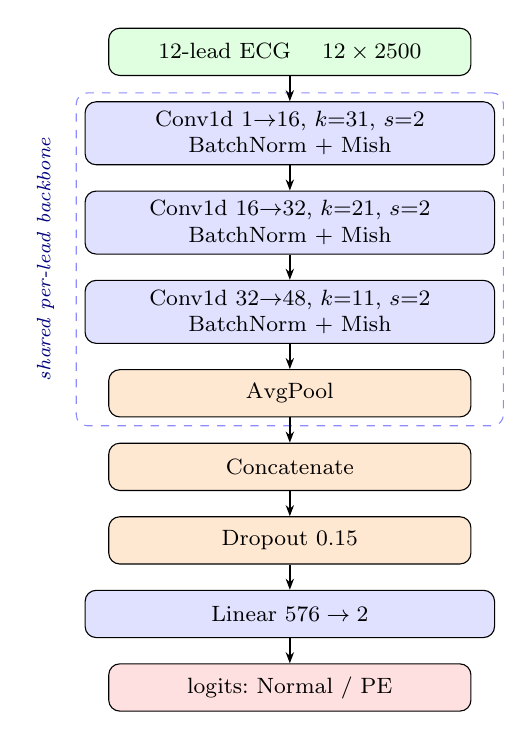
\begin{tikzpicture}[
  font=\footnotesize,
  node distance=3.2mm,
  io/.style  ={draw, rounded corners, fill=green!12,  minimum width=4.6cm, minimum height=6mm, align=center},
  conv/.style={draw, rounded corners, fill=blue!12,   minimum width=5.2cm, minimum height=8mm, align=center},
  op/.style  ={draw, rounded corners, fill=orange!18, minimum width=4.6cm, minimum height=6mm, align=center},
  arr/.style ={-{Stealth[length=4pt]}, semithick},
]
\node[io] (in) {12-lead ECG \quad $12\times2500$};
\node[conv, below=of in]  (c1)  {Conv1d $1{\to}16$,\ $k{=}31$,\ $s{=}2$ \\ BatchNorm $+$ Mish};
\node[conv, below=of c1]  (c2)  {Conv1d $16{\to}32$,\ $k{=}21$,\ $s{=}2$ \\ BatchNorm $+$ Mish};
\node[conv, below=of c2]  (c3)  {Conv1d $32{\to}48$,\ $k{=}11$,\ $s{=}2$ \\ BatchNorm $+$ Mish};
\node[op,   below=of c3]  (gap) {AvgPool};
\node[op,   below=of gap] (cat) {Concatenate};
\node[op,   below=of cat] (drop){Dropout $0.15$};
\node[conv, below=of drop, minimum height=6mm] (fc) {Linear $576 \to 2$};
\node[io,   below=of fc, fill=red!12] (out) {logits:\ Normal / PE};
\foreach \a/\b in {in/c1, c1/c2, c2/c3, c3/gap, gap/cat, cat/drop, drop/fc, fc/out}
  \draw[arr] (\a) -- (\b);
\begin{scope}[on background layer]
  \node[draw=blue!45, dashed, rounded corners, fit=(c1)(c2)(c3)(gap), inner sep=3pt] (bb) {};
\end{scope}
\node[rotate=90, anchor=south, font=\scriptsize\itshape, text=blue!50!black]
  at ([xshift=-1.5mm]bb.west) {shared per-lead backbone};
\end{tikzpicture}}
\caption{RepNet-CNN architecture ($29{,}490$ parameters). The $12\times2500$
input is reshaped to $(12,1,2500)$ so the dashed shared per-lead backbone ---
three Conv1d$\to$BatchNorm$\to$Mish stages with channel widths
$16{\to}32{\to}48$ and kernels $31,21,11$ at stride $2$ --- is applied
identically to every lead. Average pooling collapses each lead to a $48$-d
vector; the twelve are concatenated into a $576$-d representation and mapped
to Normal/PE logits by a single $\mathrm{Dropout}(0.15)$,
$\mathrm{Linear}(576,2)$ head. Sharing the backbone across all twelve leads
keeps the parameter count at $29{,}490$.}
\label{fig:arch}
\end{minipage}\hfill
\begin{minipage}[t]{0.60\textwidth}
\centering
\resizebox{!}{4.5cm}{%
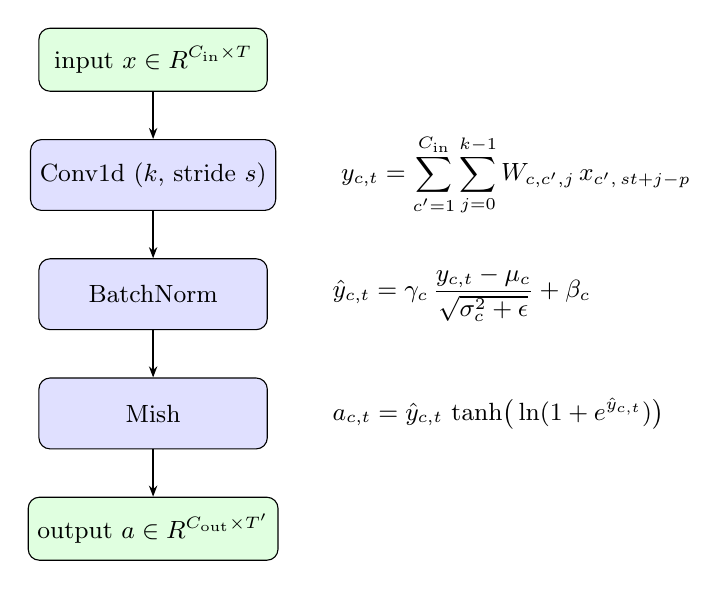
\begin{tikzpicture}[
  font=\small,
  node distance=6mm,
  op/.style={draw, rounded corners, fill=blue!12, minimum width=2.9cm, minimum height=9mm, align=center},
  io/.style={draw, rounded corners, fill=green!12, minimum width=2.9cm, minimum height=8mm, align=center},
  eq/.style={align=left},
  arr/.style={-{Stealth[length=4pt]}, semithick},
]
\node[io] (x) {input $x\in\mathbb{R}^{C_{\text{in}}\times T}$};
\node[op, below=of x]    (conv) {Conv1d ($k$, stride $s$)};
\node[op, below=of conv] (bn)   {BatchNorm};
\node[op, below=of bn]   (mish) {Mish};
\node[io, below=of mish] (a)    {output $a\in\mathbb{R}^{C_{\text{out}}\times T'}$};
\foreach \p/\q in {x/conv, conv/bn, bn/mish, mish/a} \draw[arr] (\p)--(\q);
\node[eq, right=7mm of conv] {$y_{c,t}=\displaystyle\sum_{c'=1}^{C_{\text{in}}}\sum_{j=0}^{k-1} W_{c,c',j}\,x_{c',\,st+j-p}$};
\node[eq, right=7mm of bn]   {$\hat{y}_{c,t}=\gamma_c\,\dfrac{y_{c,t}-\mu_c}{\sqrt{\sigma_c^2+\epsilon}}+\beta_c$};
\node[eq, right=7mm of mish] {$a_{c,t}=\hat{y}_{c,t}\,\tanh\!\big(\ln(1+e^{\hat{y}_{c,t}})\big)$};
\end{tikzpicture}}
\caption{One backbone block, unrolled with its governing equations
(right): a bias-free Conv1d of kernel $k$ and stride $s$, BatchNorm~\cite{ioffe_batch_2015} rescaling
by learned $\gamma_c,\beta_c$ over batch statistics $\mu_c,\sigma_c^2$, and the
Mish activation. The three stages instantiate this block with
$(k,C_{\text{out}})=(31,16),(21,32),(11,48)$ at $s=2$ throughout, the same
backbone applied to every lead in Fig.~\ref{fig:arch}.}
\label{fig:convblock}
\end{minipage}
\end{figure}

\begin{figure}[H]
\centering
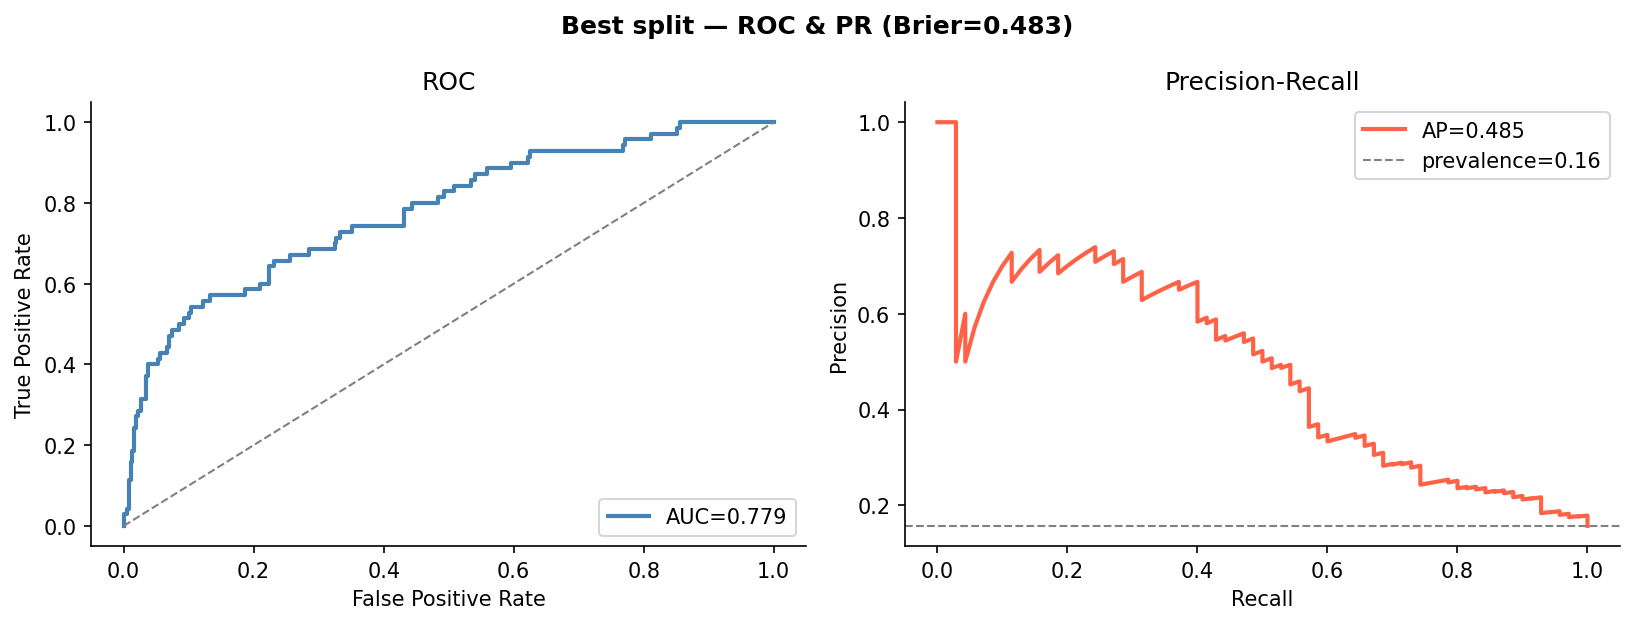
\includegraphics[width=0.74\textwidth]{figures/cnn_roc_pr.png}
\caption{Discrimination on the best of the $30$ patient-grouped splits
(AUROC $0.779$, average precision $0.485$). Left: the ROC curve. Right: the
precision--recall curve, whose $0.16$ baseline is the no-skill rate set by
preeclampsia prevalence. This split is the upper end of the
$0.709\pm0.049$ AUROC distribution reported in Table~\ref{tab:cnn-results}.}
\label{fig:cnn-roc}
\end{figure}

\begin{figure}[H]
\centering
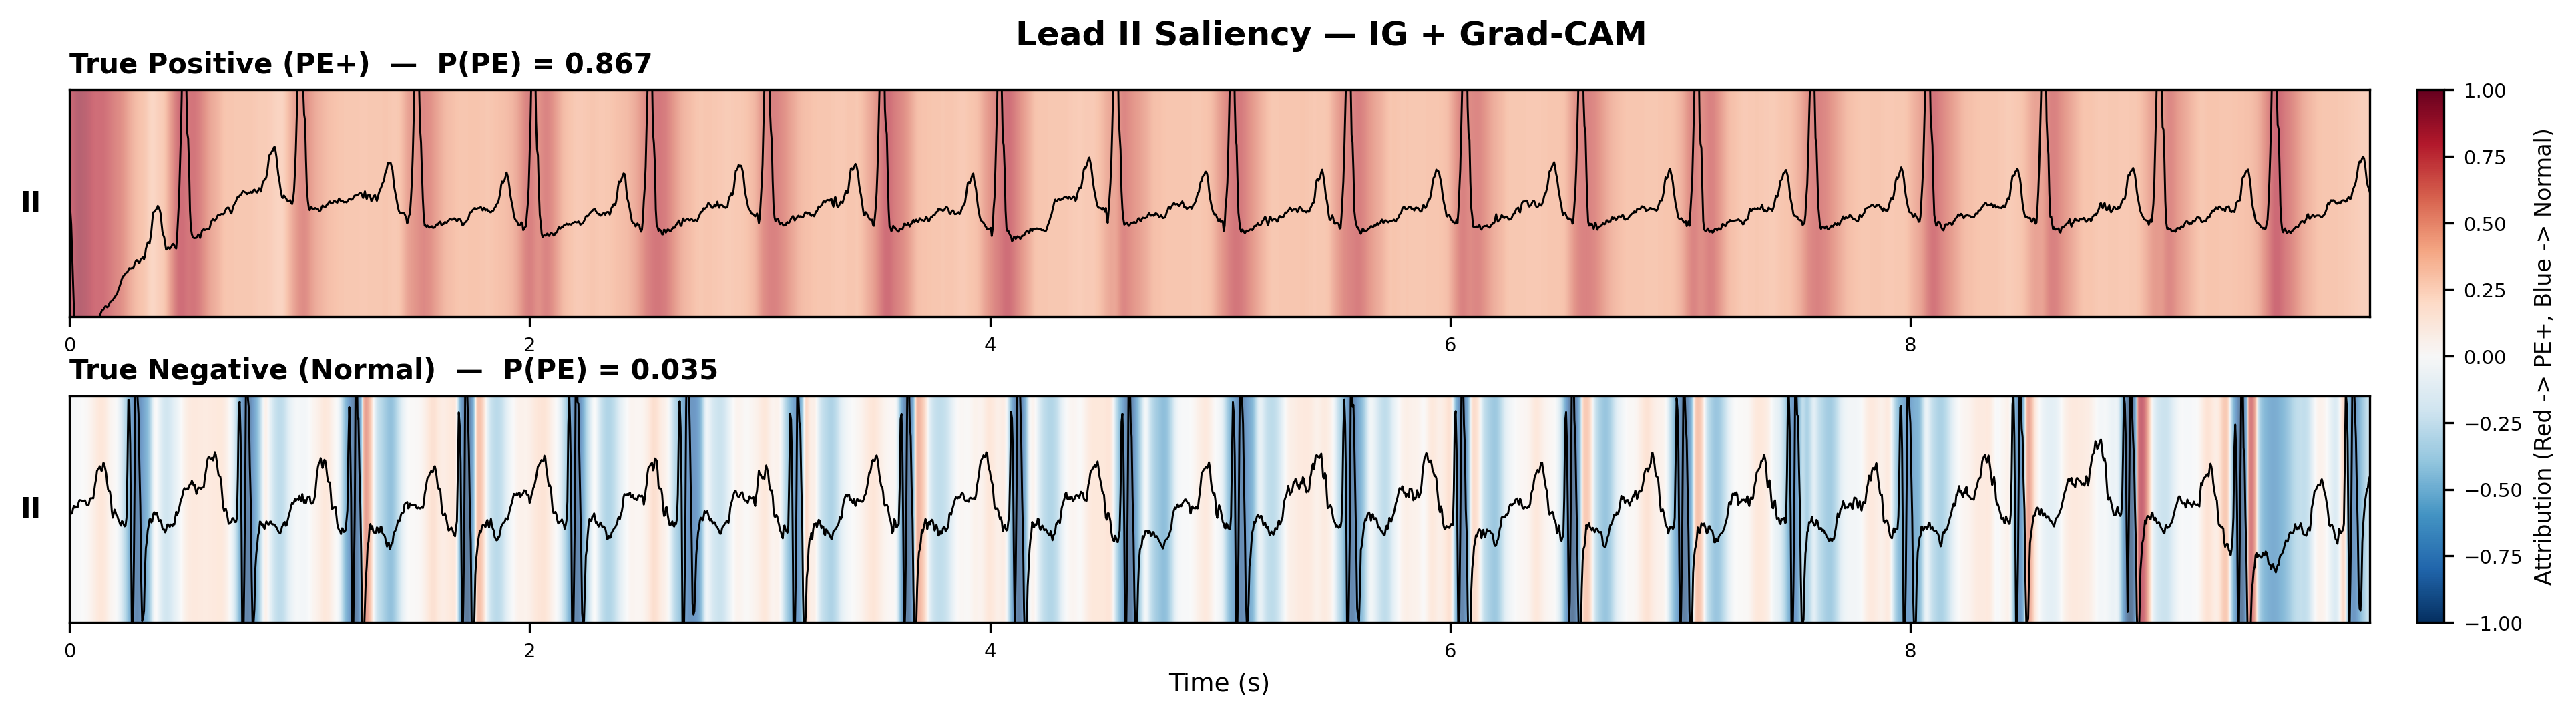
\includegraphics[width=0.86\textwidth]{figures/cnn_saliency.png}
\caption{Lead~II saliency from attributing the preeclampsia logit back to the
waveform with Integrated Gradients and Grad-CAM: red marks samples pushing the
prediction toward preeclampsia, blue toward normal. On a confident true
positive (top) the attribution concentrates on the QRS complexes and ST
segments; it reverses sign on a true negative (bottom), indicating the network
keys on clinically meaningful morphology rather than spurious artefacts.}
\label{fig:cnn-saliency}
\end{figure}

\clearpage
\section{RepNet-RF Features and Lead Importance}
\label{appendix:features}
\label{appendix:rf-imp}
\setlength{\intextsep}{3pt}
\setlength{\floatsep}{3pt}
\setlength{\textfloatsep}{3pt}

The features RepNet-RF computes with NeuroKit2~\cite{makowski_neurokit2_2021} are defined in
Table~\ref{tab:rf-neuro}, and the same quantities derived from the
GE MUSE-reported fields in Table~\ref{tab:rf-muse}. These are standard
electrocardiographic constructs~\cite{surawicz_chous_2008}, with the
repolarization-dispersion measures ($T_{pe}$, QT dispersion, and their
rate-corrected ratios) following established clinical definitions~\cite{aboshady_qtc_2025, raffaelli_pre-eclampsia_2014}. Figure~\ref{fig:rf-lead}
then counts the important engineered features per lead, and
Fig.~\ref{fig:rf-feat} how often each measurement is flagged as important
across the twelve leads.

\begin{table}[H]
\centering
\footnotesize
\renewcommand{\arraystretch}{1.2}
\begin{minipage}[t]{0.5\textwidth}
\centering
\caption{ECG features extracted with NeuroKit2.
$P_{\text{on}}/P_{\text{off}}$ are P-wave on/offsets, $R_{\text{on}}$ the QRS
onset, and $T_{\text{off}}, T_{\text{peak}}$ the T-wave offset and peak;
subscript $\ell$ ranges over the twelve leads.}
\label{tab:rf-neuro}
\vspace{2pt}
\begin{tabular}{@{}ll@{}}
\toprule
\textbf{Feature} & \textbf{Definition} \\
\midrule
$P_{\max}$ & $\max_{\ell}(P_{\text{off}}^{\ell} - P_{\text{on}}^{\ell})$ \\
$P_{\min}$ & $\min_{\ell}(P_{\text{off}}^{\ell} - P_{\text{on}}^{\ell})$ \\
P-wave dispersion & $P_{\max} - P_{\min}$ \\
QT dispersion & $\max_{\ell}(T_{\text{off}}^{\ell}{-}R_{\text{on}}^{\ell}) - \min_{\ell}(T_{\text{off}}^{\ell}{-}R_{\text{on}}^{\ell})$ \\
$T_{pe}$ interval & $\mathrm{mean}(T_{\text{off}} - T_{\text{peak}})$ \\
$T_{pe}/\mathrm{QT}$ & $T_{pe} \,/\, \mathrm{mean}(T_{\text{off}} - R_{\text{on}})$ \\
$T_{pe}/\mathrm{QTc}$ & $(T_{pe}/\mathrm{QT})\,\sqrt{\Delta R_{\text{peak}}}$ \\
ST elevation & $\mathbf{1}[\,{>}\,50\%\ \text{elevated}\,]$ \\
ST depression & $\mathbf{1}[\,{>}\,50\%\ \text{depressed}\,]$ \\
QRS axis & isoelectric or $\arctan$ method \\
T axis & isoelectric or $\arctan$ method \\
Frontal QRS--T angle & $|\,\mathrm{QRS\ axis} - \mathrm{T\ axis}\,|$ \\
\bottomrule
\end{tabular}
\end{minipage}\hfill
\begin{minipage}[t]{0.47\textwidth}
\centering
\caption{The same features from GE MUSE-reported fields. BITFLGS is the
ST-shift bit field; $\mathrm{RAxis},\mathrm{TAxis}$ are the reported axes.}
\label{tab:rf-muse}
\vspace{2pt}
\begin{tabular}{@{}ll@{}}
\toprule
\textbf{Feature} & \textbf{Definition} \\
\midrule
$P_{\max}$ & $\max_{\ell}(P_{\text{Dur}})$ \\
$P_{\min}$ & $\min_{\ell}(P_{\text{Dur}})$ \\
P-wave dispersion & $P_{\max}-P_{\min}$ \\
QT dispersion & $\max_\ell(\mathrm{QT}_\ell) - \min_\ell(\mathrm{QT}_\ell)$ \\
$T_{pe}$ interval & $T_{\text{Dur}} + T'_{\text{Dur}} - \mathrm{STEtoTPeak}$ \\
$T_{pe}/\mathrm{QT}$ & $T_{pe}\text{ interval} \,/\, \mathrm{QT}$ \\
$T_{pe}/\mathrm{QTc}$ & $(T_{pe}/\mathrm{QT})\,\sqrt{\mathrm{RR}}$ \\
ST elevation & $(\mathrm{BITFLGS}\;\&\;8)\neq0$ \\
ST depression & $(\mathrm{BITFLGS}\;\&\;4)\neq0$ \\
QRS axis & $\mathrm{RAxis}$ \\
T axis & $\mathrm{TAxis}$ \\
Frontal QRS--T angle & $|\,\mathrm{RAxis}-\mathrm{TAxis}\,|$ \\
\bottomrule
\end{tabular}
\end{minipage}
\end{table}

\begin{figure}[H]
\centering
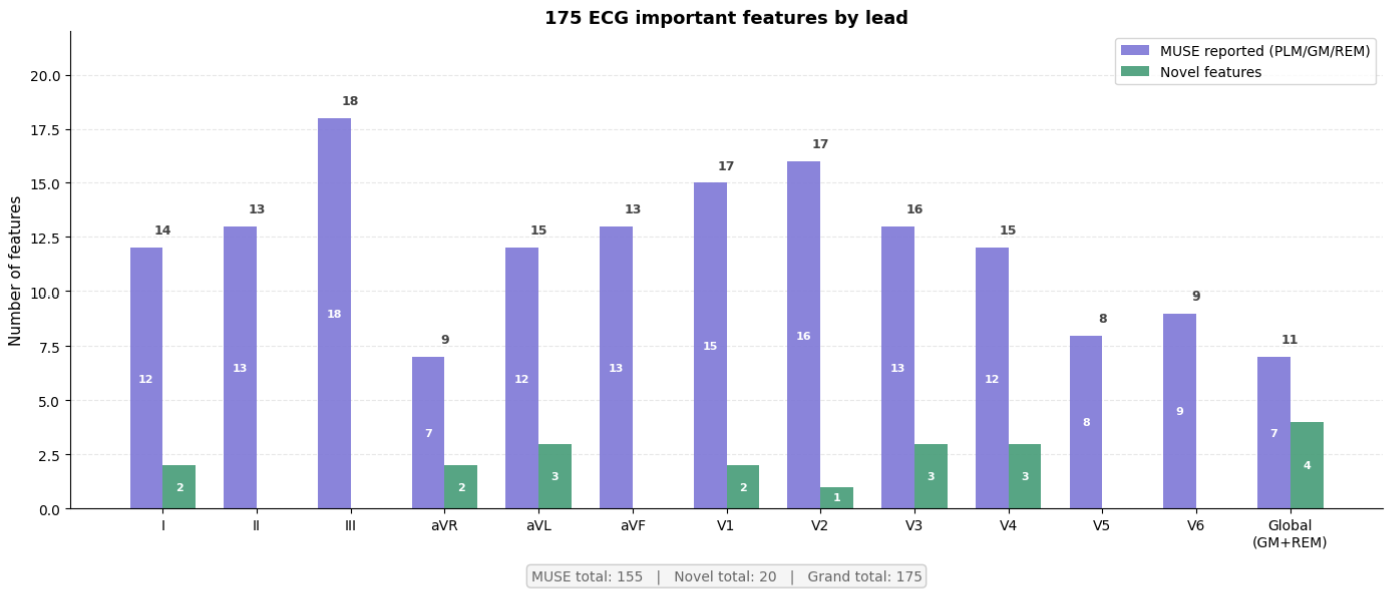
\includegraphics[width=0.62\textwidth]{figures/rf_lead_importance.png}
\caption{Count of important engineered features per lead for RepNet-RF, split
into MUSE-reported and novel (NeuroKit-derived) features.}
\label{fig:rf-lead}
\end{figure}

\begin{figure}[H]
\centering
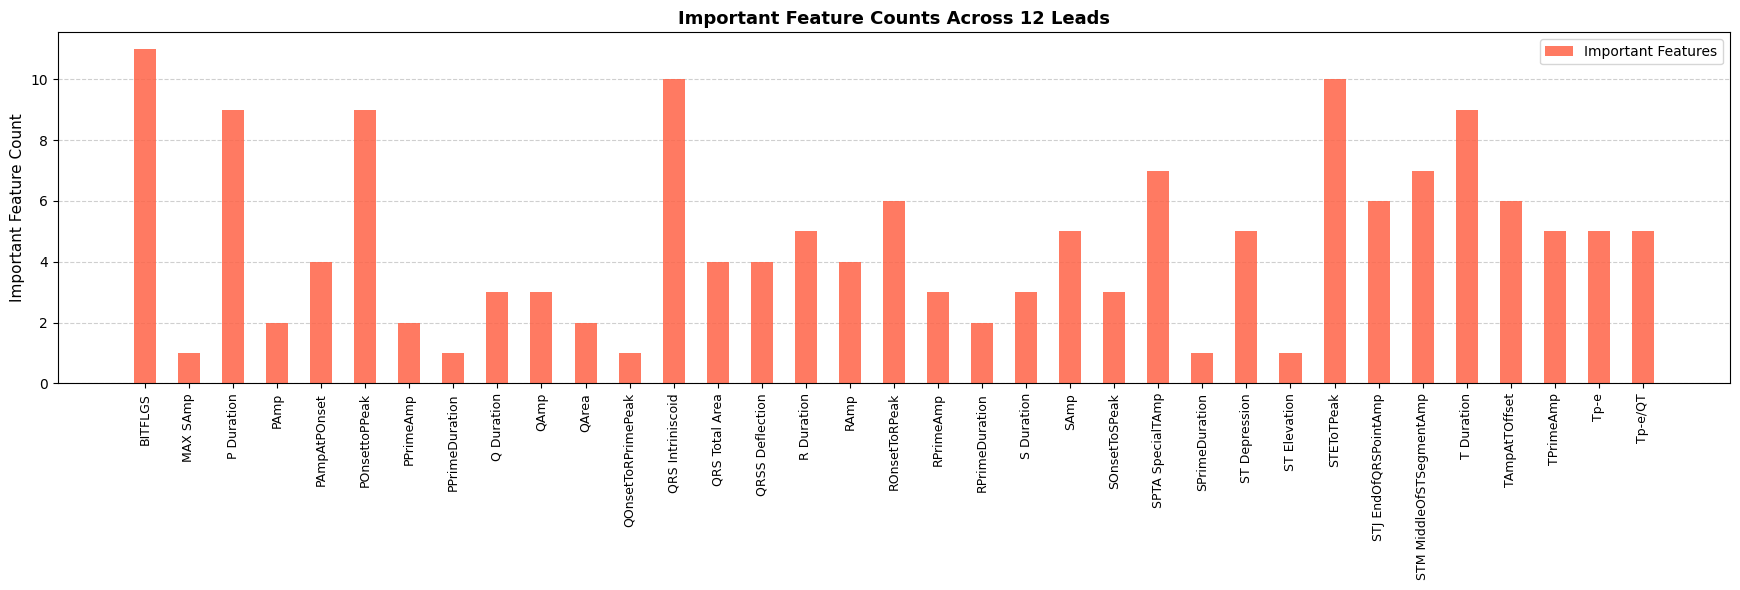
\includegraphics[width=0.72\textwidth]{figures/rf_feature_importance.png}
\caption{How often each engineered measurement is flagged as important across
the twelve leads.}
\label{fig:rf-feat}
\end{figure}

\end{document}
